\section{Introdu��o}

\begin{frame}
\frametitle{\alert{Pr�ximos Slides}}
	\beamerdefaultoverlayspecification{<+->}
	
		\begin{enumerate}
			\item Introdu��o
			\item Motiva��o
			\item Justificativa
			\item Objetivos do Trabalho
		\end{enumerate}

	\beamerdefaultoverlayspecification{<*>}
\end{frame}

\subsection{Motiva��o}

\begin{frame}
  \frametitle{Motiva��o}

		\begin{itemize}
		  \item Engenhosidade e n�mero crescente das amea�as virtuais.\\
			  		Pesquisas dizem que \textbf{83\% das operadoras} de telefonia m�vel no mundo foram v�timas de ataques em seus dispositivos.
			\item Entre os anos de \textbf{2007} para \textbf{2008} surgiram \textbf{350 tipos de malwares} diferentes para dispositivos m�veis.
		\end{itemize}
			
\end{frame}

\begin{frame}
  \frametitle{Motiva��o}
  \framesubtitle{10\textsuperscript{\d a} Pesquisa realizada em 2007 pela M�dulo Security.}

			\begin{figure}[htbp]
				\centering
					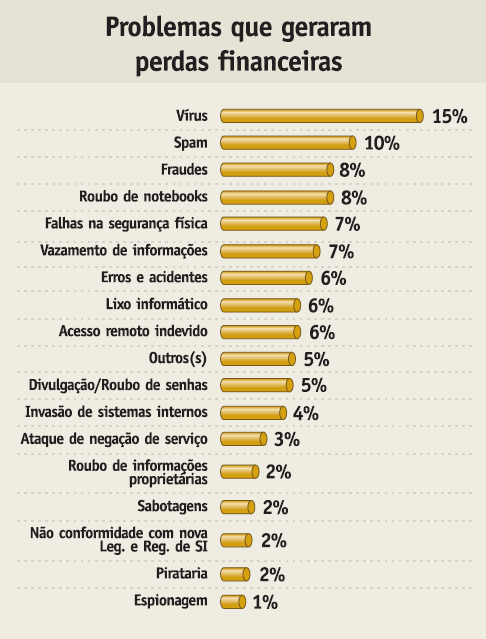
\includegraphics[width=0.40\textwidth]{../Pictures/Baixa/Estatistica_Problemas.png}
				\label{fig:Estatistica_Problemas}
			\end{figure}

\end{frame}


%_______________________________________________________________________
\subsection{Justificativa}


\begin{frame}
  \frametitle{Motiva��o}

			\begin{figure}[htbp]
				\centering
					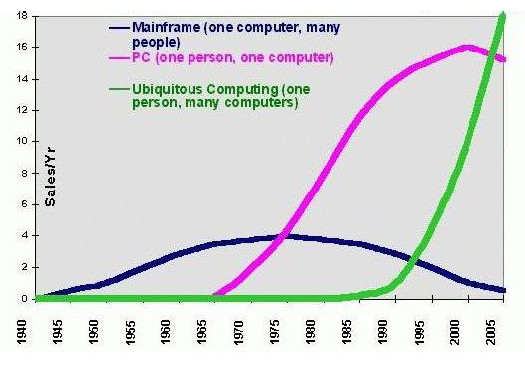
\includegraphics[width=0.80\textwidth]{../Pictures/Baixa/Grafico_Weiser.png}
				\label{fig:Grafico_Weiser}
			\end{figure}

\end{frame}

\begin{frame}
  \frametitle{Porque usar um Firewall?}
  
	\begin{center} 
			\LARGE \textbf{Conectar-se � Internet sem um \alert{Firewall} � como deixar as chaves do carro no contato, o motor ligado e as portas destravadas enquanto voc� vai �s compras !}
	\end{center}

\end{frame}


\begin{frame}[allowframebreaks]
  \frametitle{Porque usar um Firewall?}	

		\begin{itemize}
			\item \textbf{Quanto tempo seu \alert{Dispositivo M�vel} passa completamente \alert{DESLIGADO} ?!}
			% \item	A mobilidade pode se tornar um grande problema de seguran�a!
			\item Redes wireless abertas tem se tornado cada vez mais comum.			
			\item	Dispositivos M�veis possuem uma variedade maior de interfaces de comunica��o:			
					\begin{enumerate}
						\item Bluetooth;
						\item Wi-Fi;
						\item USB;
						\item EDGE;
						\item GPRS;
						\item Infra-vermelho 
					\end{enumerate}					
		\end{itemize}

\end{frame}


\begin{frame}
  \frametitle{Porque usar um Firewall?}				
				
	\begin{itemize}
			\item Imagine um Cavalo de Tr�ia que foi instalado junto com aquele seu toque predileto que voc� baixou da internet, e este Trojan envia suas senhas enquanto voc� acessa \alert{E-mail e Internet Banking} do seu Dispositivo M�vel.			
			\item Imagine que o simples fato de acessar um site atrav�s de seu Dispositivo M�vel cause o \textbf{apagamento} de todos os seus dados pessoais (Agenda, Compromissos etc)...
	\end{itemize}

\end{frame}


\begin{frame}
  \frametitle{Porque usar um Firewall?}
			\begin{itemize}
				\item Imagine voc� esquecer o \textbf{Bluetooth} ligado e outras pessoas acessar seus dados pessoais.
				\item Imagine um Worm como o \textbf{Blaster} para Dispositivos M�veis, que cause uma \textbf{Nega��o} nos servi�os de Telefonia m�vel...
								
			\end{itemize}
\end{frame}

				
\begin{frame}
  \frametitle{Porque usar um Firewall?}

			\begin{itemize}
				\item \alert{Sem} um Firewall voc� est� sujeito a v�rios ataques:
						\begin{enumerate}
							\item V�rus;
							\item Worms;
							\item Cavalos de Tr�ia;
							\item SynFlood;
							\item Ping of Death;
							\item Smurf;							
							\item Outros...
						\end{enumerate} 			
			\end{itemize}		
  
\end{frame}


%_______________________________________________________________________
\subsection{Objetivos do Trabalho}
\begin{frame}
  \frametitle{Objetivos do Trabalho?}

	\begin{figure}[htbp]
			\centering
				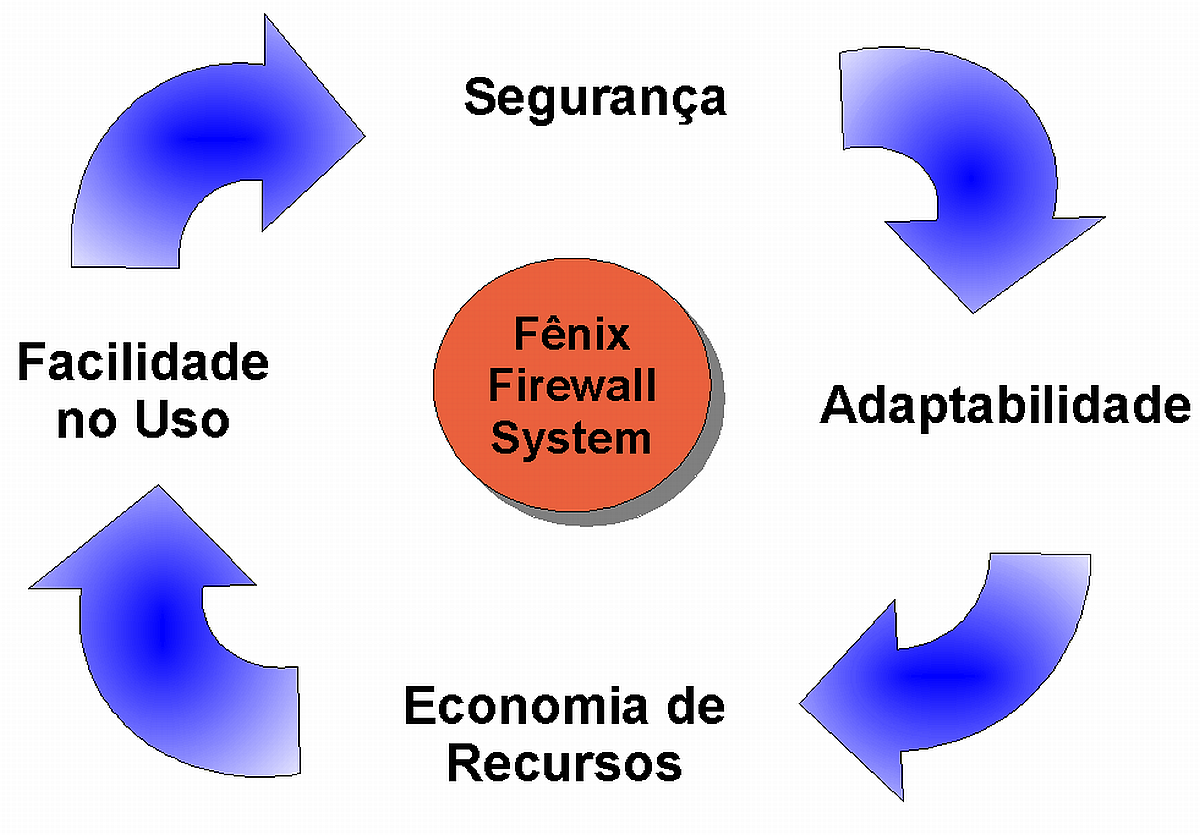
\includegraphics[width=0.80\textwidth]{../Pictures/Baixa/Ciclo_Fenix.png}
				\label{fig:Ciclo_Fenix}
			\end{figure}

\end{frame}